\documentclass{article}

\usepackage[vmargin=2cm]{geometry}

\usepackage{wx672bib}
\addbibresource{bib/net.bib}
\addbibresource{bib/rfc.bib}

\usepackage{wx672hyperref}
\usepackage{amsmath,amsfonts,amssymb}
\usepackage{graphicx}
\graphicspath{{./figs/}{../figs/}{./}{../}}
\usepackage{capt-of}
\usepackage{enumitem}
\setlist{nosep}


\author{WANG Xiaolin\\\emph{\small wx672ster+net@gmail.com}}
\date{\today}
\title{Computer Networks Seminar Minutes}

\hypersetup{
  pdfauthor={WANG Xiaolin},
  pdftitle={Computer Networks Seminar Minutes},
  pdflang={English}}

\begin{document}

\maketitle
\tableofcontents

\vspace{1em}

\begin{description}
\item[Class schedule]\, 
  \begin{itemize}
  \item 10am, every Monday
  \item 2pm, every other Tuesday starting from \emph{2020-04-21 Tue}
  \item 10am, every other Wednesday starting from \emph{2020-04-29 Wed}
  \end{itemize}
\item[Course website] \url{https://cs6.swfu.edu.cn/moodle/course/view.php?id=4}
\item[Local ebooks] \url{https://cs6.swfu.edu.cn/calibre}
\end{description}

\printbibliography

\section{2020-04-20 Mon}

\subsection[No questions?]{New in this subject, knowing nothing yet, how can
  we ask you question?}
\label{sec:noquestions}

Good point. You've learnt nothing yet. So there should be full of questions in your
head. But why can't you pop up a single question? It's because you're expecting that all
the questions can be answered automatically in the class.

Why bother to think of a question if the answer is so cheap? Thus you don't think.
Learning is about thinking. But you seem happy with learning without thinking.  We come to
class, we listen, and we forget everything after class. We've been happily calling this
\emph{learning} for more than ten years.  You see, we are happy to cheat ourself
sometimes.

\subsection[No video?]{Why no video tutorials? It's more easy to understand our subject.}
\label{sec:novideo}

As a Chinese, you know my oral English is terrible. Honestly it's not so practical to
expect a good video from me. Hopefully, there are plenty of video tutorials available on
youtube.

\paragraph{No, sir, we want teaching from you. We need online live class from you. I think
  it is best for us.}

Right, you want \emph{teaching}, what about \texttt{learning}?  What do you mean
\emph{teaching from me}? Two hours of live video, twice a week? Do you really think this
is \emph{teaching} and \emph{learning}? If you really want to watch videos, why don't you
do it after class so that we can spend these 2 hours more efficiently?

Let's don't pretend to be teaching and learning. Stop cheating ourselves.  If you really
want to learn, learn it in the right way. So, what's the right way?
\begin{enumerate}
\item You watch online videos after class if you like. Then,
\item You have to read the books. Even if you watched a lot of videos, you still need to
  read the books. Even you listened to the lectures in the class, you still need to read
  the books after class.
\item When you find a problem, you try solving it by googling and reading. What if you
  can't solve it?
\item You ask me in the proper way like this in the forum:
  \begin{enumerate}
  \item What was I trying to do?
  \item How did I do it? (steps)
  \item The expected output? The real output?
  \item How did I try to solve it? (steps, books, web links)
  \item How many hours did I strugle on it?
  \end{enumerate}
  Forum: \url{https://cs6.swfu.edu.cn/moodle/mod/forum/view.php?id=98}
\end{enumerate}

\subsection[How to begin?]{How to begin my study? What should we do first?}
\label{sec:begin}

You go through the slides, handouts, textbooks, videos, and come here with your questions.

\paragraph{When come here with my question, sir? Class time?} Any time.

\paragraph{The moodle app doesn't work?} Try it in a web browser on a PC.

\subsection[What is networking?]{What is computer networking? How it works?}
\label{sec:whatis}

Obviously, we have to connect the computers, devices together, right? And there is
more. Network is not about connection, it's about communication.  Over the network,
computers can talk to each other.

Want to know more? The whole purpose of this course is to explain more on it.  What's it
look like? How they communicate? Etc.

\paragraph{Sir, can you explain topology. I can't understand it properly.}

Well, you can say it's the \emph{shape} of a network. Some popular topologies
are shown on page 23 of the slides.

\section{2020-04-21 Tue}

\subsection[What's in today's class?]{What will we learn today? Sir, today how can we
  start the class? And which topic we study? We are new in this subject.}
\label{sec:today}

What have you read before today? Nothing? Then you shouldn't be here because you
are not here to learn something, instead, you are here pretending to learn something.

You come to class, you listen. After class you don't do anything and forget everything.
Then, you come to class again. This is not learning, this is cheating, cheating yourself.

\subsection[Not comfortable with chatting class?]{I'm not comfortable with this chatting
  class. we need live video class to understand and explanation. I'm too uneasy wtih this
  system. Actually, we don't understand how should we study in this system. Sir, I think
  we need your lecture video with your lecture slides, then it would be better. If you
  provide your lecture video on your lecture slide it will be more clear to us.}
\label{sec:comfortable}

I'm not comfortable with this situation either. And I don't think it will be
more comfortable even if we are face to face in a classroom. You know why? See my answer
to question~\ref{sec:today}, question~\ref{sec:noquestions}, and question~\ref{sec:novideo}.

\paragraph{Don't know where to start.}

Why don't start with the first slide?  Have you done that? why not? because I want video,
right? you got video on the web, then what? I want \emph{your} video. For what? Am I a movie
star? Again, do you really want to learn, or just pretend to learn? You paid a lot of
money for this college education, right? What do you really want? My videos?

Hope this is the last time we talk about the videos. I'm not a movie star. And my oral
English is not good. And you can get lots of excellent video tutorials on the web. Then,
you still insist on my video, why?  What's wrong with the open course videos from MIT,
Harvard, Stanford, UCLA?

Actually you don't hate this chatting class, you hate \emph{learning}. Learning is not
about being lectured in the classroom, not about being taught the answers/solutions to the
questions. Learning is not about the answer. It's the process of getting the answer.  You
seem have never been through this process before. You hate this process because you
have to read the slides, handouts, textbooks, and find the answer all by yourself. That's
too hard and too boring and too painful to go through it.

Yes, you prefer teaching to learning because teaching is less painfull. But what have you
got from it? Like I said, if you don't do anything after class, you got nothing.  Yes,
teaching is of course helpful, but only if you learn. All you have gained from school in
the past 10 years is from painful learning. That's why it's said no pain no gain.

Here is an excellent scientific paper about teaching and learning, you really should give
it a look.
\begin{itemize}
\item \url{https://journals.physiology.org/doi/full/10.1152/advan.00061.2005}
\end{itemize}

So, in our class, if you learn, I help. If not learn, you fail.

\subsection[Google before ask?]{Sir, what is TCP? Is IP and TCP the same?  What is LAN? Sir, please tell us about this subject.}

Good question. But next time, before you ask, you should google it first.

\paragraph{How can I use google in China?}

This is a real question. For now, if you can't google, you can use \url{bing.com} instead.

\paragraph{Sir, if Google is everything, why we come to China?}

Figure it out yourself. We don't have google in China. Do we have network experts in
China? Maybe, but you can find more outside China, right? Why you are here?  For what? For
my class videos?

Google is the best library in the world. If you want to learn anything, you really should
go to library. You really don't have to go to college.

Well, you are here. If you want my help, I will do my best. If you want my video, you are
wasting your tuition fees. You should go Hollywood for movie stars.

\paragraph{Sir, Google and YouTube is not solution to everything. I hope we can be
  comfortable with live explanation class and I hope everyone will be comfortable with
  that. If you want then we create an account on ding talk app and we started our class
  there comfortably.}

Actually I don't see any solutions for you if you just want to go to school, but don't
really want to learn anything.
  
\paragraph{Sir, please tell us, from where we should start in lecture slide?}

How about start with page one? Any question with p1? if not, go to p2, p3, p4... Go
through the slides until you find a question.

\subsection[How to ask?]{Teacher, can you explain us about ethernet and how it works?}

Good. Next time, ask question like this: Sir,
\begin{enumerate}
\item I want to figure out how ethernet works. Then,
\item I googled, and read some articles about it. But,
\item I'm still a bit confused about ``blah blah blah''.
\item These are the web links I visited. These are the books I read...
\item I struggled on this question for (how many?) hours.
\end{enumerate}
This is called \emph{learning}.

About ethernet, your first reading should be rfc1180 \citetitle{rfc1180}.
\begin{itemize}
\item \url{https://tools.ietf.org/html/rfc1180}
\end{itemize}
Lots of things you should do before you come to class, right?

\paragraph{Weblinks share with you via wechat or here?}

Here. If you want to share pictures, go with wechat.

\subsection[Homework?]{What is our homework?}

Your homework is on page 4 of the slides. You haven't been there, have you?

Don't forget (or ignore) the homework. It's extremely important. Your final result heavily
depends on it.

\begin{itemize}
\item forum: \url{https://cs6.swfu.edu.cn/moodle/mod/forum/view.php?id=98}
\end{itemize}

\paragraph{Homework: Meanwhile, what happened in China? what do you mean in this line sir?
  about china Modernisation?}

You don't have to worry about that line. It's for Chinese students. That's just to remind
the Chinese students how far China is left behind the world. For you, maybe you are more
interested in finding out things happened in Bangladesh.

\paragraph{Sir, there are 5 questions in page 4, but I can not understand that those
  questions on which topic?}

Any topic you like, preferably about networking. The point of the homework is to learn
\emph{how to learn in the right way}.

You have to submit your homework at least once a week.

\paragraph{Why this homework?}
\begin{itemize}
\item Try Linux
\item Get a gmail account
\item Use Google calendar
\item Use Youtube
\end{itemize}

\begin{enumerate}
\item Try Linux. Because all the network administrators (should) use Linux/Unix. All our
  networking commands are based on Linux/Unix. We don't use Windows. I've been using Linux
  for more than 20 years. Believe me, it's great. If you want to find a good job, make
  good money, Linux is your choice.
\item For Chinese students, I encourage them to use google as much as possible.
\end{enumerate}


\subsection[Exam?]{Want to know something about the exam?}
\label{sec:exam}

Most of the questions on the exampaper will come from your questions and homeworks. Well,
if you don't ask any questions, and don't do the homework well, the exampaper won't be
empty. I'll have to invent questions myself. That's not good for you, right?

\subsection[Linux?]{We don't know anything about Linux/Unix.}
\label{sec:linux}

Then you learn it. That's why you come to college.
  
Linux is a Unix-like, open source and community-developed operating system for computers,
servers, mainframes, mobile devices and embedded devices. It is supported on almost every
major computer platform including x86, ARM and SPARC, making it one of the most widely
supported operating systems. (Thanks to ASIF UD)

\begin{itemize}
\item Installation guide:
  \url{https://cs6.swfu.edu.cn/~wx672/debian-install/install-en.html}
\end{itemize}
Follow this installation guide you will have a linux system looks exactly the same as I
am currently using.

If you encounter any problems during installation, go to the forum, ask a proper
question. That's a perfect homework.

\subsubsection{Linux books?}
\label{sec:linux-books}

You don't need a book to learn how to ride a bike, right? Just like a bike, Linux is
merely another tool used for solving some problems. If you keep using it for your daily
work, you will get used to it pretty soon.

\paragraph{CLI is everything.}

You should focus on the CLI (Command Line Interface) when you use Linux.  In the computer
world, you can live without a mouse, but you can't live without a keyboard. For example,
as a general user, can you write an email entirely with a mouse?  Well, it's possible to
do it with an on-screen virtual keyboard. Do you really enjoy that?

As a sys-admin, do you prefer to manage the remote servers with mouse clicking? If you say
yes, I'd not hire you as my sys-admin. Why?

\begin{description}
\item[System stability] To support mouse clicking, the remote servers must have GUI
  (Graphical User Interface) installed. You know, more codes more bugs. GUI is a huge
  software with enormous lines of codes. If you install GUI programs on your server, lots
  of software bugs will come with it. That makes your server weak.
  
\item[Resource efficiency] A server is supposed to serve the users rather than the
  sys-admin. However, the mouse enabled resource-consuming GUI programs can only serve the
  sys-admin. For example, the web servers don't need GUI programs to satisfy the users'
  requests. 
  
\item[Network efficiency] Operating on the remote server with a CLI is much more efficient
  than that with a mouse. For example, if you want to list files in a folder,
  \begin{itemize}
  \item with CLI, you just send `\texttt{ls}' to the server. That's just 2 bytes. Soon the
    server will return you the file list in plain text. That's about some hundreds of bytes.
  \item with GUI, your every mouse click on the file manager window will trigger the
    transfer of the window image between remote and local. And each image is at least
    serveral kilobytes in size. Obviously, the CLI way is much more bandwidth efficient
    than the GUI way.
  \end{itemize}
\end{description}

Linux systems are widely used as servers. When you are learning Linux, you should do it
like a real sys-admin, keep both of your hands on the keyboard, and better forget your
mouse and touchpad.

\paragraph{Don't I need a book to learn CLI?}

Yes, sometimes it'd be helpful to have something to read. That's why every *nix
system comes with a comprehensive manual system. For example, if you want to know more
about the command `\texttt{ls}', you can just type `\texttt{man ls}'.

But the man pages are so lengthy and boring to read. It's really not easy to stand
it. Right, I agree, that's why I never really read the man pages. Instead, I search in
it. For example, when you are doing `\texttt{man ls}', you can type slash (`\texttt{/}')
followed by any word you want to search, so that you can find the information you want
very quick.

Well, there are tons of Linux books available. And they are there for a reason, right? Of
course. But before reading any books, I prefer googling first. If Google can't help, here
comes the books:
\begin{description}
\item[bash] This is the default shell on Linux.
  \begin{itemize}
  \item bash cookbook: \url{https://cs6.swfu.edu.cn/calibre/get/PDF/170/calibre}
  \item Advanced bash-scripting guide: \url{https://tldp.org/LDP/abs/html/}
  \end{itemize}
\item[tmux] A powerful terminal multiplexer that I cannot live without.
  \begin{itemize}
  \item \url{https://cs6.swfu.edu.cn/calibre/get/PDF/144/calibre}
  \end{itemize}
\item[vim] One of the most powerful editor in the world. But before you read the books,
  you really should try the command `\texttt{vimtutor}' first.
  \begin{itemize}
  \item \url{https://cs6.swfu.edu.cn/calibre/get/PDF/172/calibre}
  \end{itemize}
\end{description}



\subsection{After class?}
\label{sec:after-class}

Everyone, before you come to next class (Monday), make sure you've read rfc1180.  You will
have lots of questions while you are reading rfc1180. Then what? You google.  And if you
can't find the answer, you come to the forum, ask a proper question. That makes it a
perfect homework, right?



\section{2020-04-26 Sun}
\label{sec:2020-04-26}

\subsection{Programming on Linux?}
\label{sec:programming-linux}

\begin{description}
\item[How many programming languages are supported on Linux?] Actually I don't know which
  language is not supported on Linux. It's safe to say all the languages you know are well
  supported on Linux.
\item[Which languages should I learn?] C, Java, Python.
  \begin{description}
  \item[C] By far, C is the only language that used in system programming.
  \item[Java] The most popular programming language in the world. C++, C\# has the same
    programming concept as Java. But Java is the most popular one. If you learn Java well,
    it's very easy to switch to C++ or C\#.
  \item[Python] Perhaps the most popular one in the near future.
  \end{description}
  If you want to learn more about the popularity of programming languages, you should
  check TIOBE index (\url{https://www.tiobe.com/tiobe-index/}).
\item[How do I start C/C++ coding on Linux?] If I were you, I'd start with googling
  `\texttt{c tutorial linux}'.
\end{description}


\subsection{What's a protocol?}
\label{sec:whats-protocol}

Before we have computers, we have protocols already. It's something agreed by
two or more people so that they can cooperate with each other.

If two or more computers want to cooperate with (send data to) each other, they have to do
that as we people do. That's the network protocols (a set of rules) that are agreed
(understood) by all the computers.

\paragraph{What's a computer network?}

Two things:
\begin{enumerate}
\item They have to be connected to one another in some way (wired or wireless);
\item They have to follow the same set of rules so as to talk to each other.
\end{enumerate}

\subsection{What's in a protocol?}
\label{sec:whats-in-protocol}

Every problem that can bug the communication must be addressed in whichever
protocol. For example:
\begin{itemize}
\item I only want to send data to one of them. How to distinguish them? (Every computer
  should have an identifier, e.g. address)
\item How do I know where is the beginning of the data message? Where is the end of the message?
  (The data format should be standardized)
\item How do I know my message is received by the other end? (Need a mechanism to make
  sure that, e.g. ACK)
\item I sent him two letters. But only got one reply. Where's the other one? (What to do
  if data lost)
\item \ldots
\end{itemize}

There are lots of details need to be taken care of. Every detail need to be addressed as
an article (rule) in whichever protocol.  

\subsubsection{About IP address}
\label{sec:about-ip-address}

An IP address is very similar to the mail address we use in our daily life. In real life,
the address is an identifier of a geographical position on the earth.
\begin{itemize}
\item An address can only be assigned to one place. But one place can have many
  addresses. Same applys to computers,
\item An IP address can only be assigned to one computer, while a computer can have more
  than one addresses.
\end{itemize}
When you try to understand the concepts of Internet, you should use your common sense. 


\subsection{How many protocols are there?}

Thousands RFCs made by IETF. Apart from IETF, there are ISO, ITU, IEEE\ldots
Lots of standard makers.

So, who we follow? We follow IETF. TCP/IP is the set of protocols that published
by IETF. As a beginner, the most basic RFCs you need to know:
\begin{itemize}
\item \citetitle[RFC 1180]{rfc1180}
\item \citetitle[RFC 791]{rfc791}
\item \citetitle[RFC 793]{rfc793}
\end{itemize}

\subsection[Why layered design?]{Why there are so many layers? What's the point to have a
  layered design?}

You should read the textbook \citetitle[Sec.~1.3]{tanenbaum2011computer}.
Key points:
\begin{itemize}
\item Modular design, divide a huge complex problem into several small simple
  problems. This can reduce the design complexity.
\item The relationship between adjacent layers (service, physical)
  \begin{itemize}
  \item Each layer offers services to its upper layer through \emph{interfaces} (function
    calls in software term).
  \item Each layer is a blackbox to other layers.
  \end{itemize}
\item the relationship between peer layers (protocol, logical)
  \begin{itemize}
  \item When layer $n$ on one machine talks with layer $n$ on another machine, the rules
    and conventions used in this conversation are collectively known as layer $n$ protocol.
  \end{itemize}
\end{itemize}

\subsubsection{How many layers should we have?}
\label{sec:how-many-layers}

The ISO OSI/RM has 7 layers, while the TCP/IP stack has only 4 layers. When it's taught in class, we usually take 5 layers. There're also network designed with 2 or 3 layers.

Layered design is kind of modular design of software. For example, if you have a huge
project to do, you usually divid it in to several small jobs so that each group of people
can handle one small job. So, how many small jobs you want to have? ISO says 7, IETF says
4, teachers prefer 5. the IETF one (TCP/IP) is the most popular one anyway.

The presentation layer and session layer of the OSI/RM are usually merged into the Application layer of 4/5 layer models.

\section{2020-04-27 Mon}
\label{sec:2020-04-27-1}

\subsection{Linux commands?}
\label{sec:linux-commands}

There are a bunch of Linux commands that you should learn so that you can survive at the
command line. How to learn it? Easy.
\begin{itemize}
\item
  \url{https://cs6.swfu.edu.cn/~wx672/lecture_notes/linux/bash/shell_basics.html}. This is
  a very brief introduction to bash commands. You go through it, whenever have trouble,
  you google. For example, you want to know more about the command \texttt{cat}, you can
  \begin{itemize}
  \item google `\texttt{linux cat tutorial}'. Similarly you can,
  \item google `\texttt{linux command line tutorial}'
  \item google `\texttt{linux bash tutorial}'
  \end{itemize}
\end{itemize}

\subsubsection{What's bash?}
\label{sec:whats-bash}

Well, you should google `\texttt{linux bash}'. To make it short, bash is the default
\emph{shell} on Linux. So, what's a shell? As shown in Fig.~\ref{fig:os}, a computer
system has 2 parts, hardware and software. And the software part can be divided into two
parts, the kernel (operating system), and the shell (application programs). And back to
1970s, the only application program available was the CLI. Today we have tons of GUI
programs available, but we still call the CLI \emph{the shell}. That's the Unix tradition.
So, when we talk about the shell or the CLI or bash, we are actually talking about the
same thing.

\begin{figure}
  \centering
  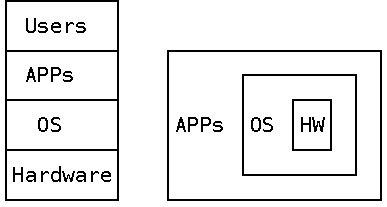
\includegraphics[width=.3\textwidth]{os}
  \caption{A computer system\label{fig:os}}  
\end{figure}

\subsubsection{What's tmux?}
\label{sec:whats-tmux}

It's a terminal multiplexer. What's a multiplexer? It's very much like kill many birds
with one stone. You open one terminal window, and use it as you have many windows.
\begin{itemize}
\item google `\texttt{tmux tutorial}'. 
\item \texttt{sudo apt install tmux}
\end{itemize}

\subsection{How to ask a question properly?}
\label{sec:how-ask-question}

Here are some wrong questions:
\begin{itemize}
\item Sir, I can not understand (\emph{understand what?})
\item My first question is about the Ethernet (\emph{what exactly is your question?})
\item Sir, what is a multiplexer? (\emph{why don't google it first?})
\item Sir, I am reading daily in short lesson, I also don’t understand clearly. (\emph{about what?})
\end{itemize}

You are not able to ask a proper question because you haven't done enough work (thinking,
reading, research) on it. You don't have to actually solve that problem, but you have to
try it hard until you can ask a real clear question. If you are able to ask clear
questions, your question is at least 50\% solved. There is a very popular article
\href{http://www.catb.org/~esr/faqs/smart-questions.html}{\emph{How To Ask Questions The
    Smart Way}}. Everybody should read it seriously.
\begin{itemize}
\item \url{http://www.catb.org/~esr/faqs/smart-questions.html}
\end{itemize}

\subsubsection{I read rfc1180, but still can't ask a question. Why?}
\label{sec:i-read-it}

If you've already read rfc1180, and still got no questions, that's most probably you read it in
the wrong way. For example, if you want to understand the Ethernet, you should
\begin{enumerate}
\item read the Ethernet part of rfc1180. After finish reading,
\item you try explain it in your own words. If you cannot explain it clearly,
\item you read it again to find out where and why you cannot explain it. If it's still
  hard to understand,
\item you google `\texttt{what is ethernet}'. After this, still confused?
\item try write down a clear question. If you can't,
\item you read rfc1180 and google `\texttt{what is ethernet}' again until you can ask a
  proper question.
\end{enumerate}

One week is past. Seems you have very little progress in your readings. Everyone of you.
The answer about Ethernet is just in rfc1180. And it's not very hard to read because it's
not written for the professionals. It's just a tutorial for normal people. Why don't read
it?

\paragraph{Okay, I'll read it. But what a teacher for?}

The teacher is not an answer machine. My job is not suppose to give whatever answers you
want. Instead, my job is to help you do your learning, is to guide your learning to the
right direction in the right way. If you are not willing to learn, I can't help.

\section{2020-04-29 Wed}
\label{sec:2020-04-29}

\subsection[LAN vs. MAN?]{Which one is LAN? Which one is MAN?}
\label{sec:which-one-lan}

The network could be very large, could also be very small. The large network is actually
composed of many small networks. The MAN is a huge city wide network which is made up of
many smaller networks. LAN, as you said, is a very small network, like an office network,
or home network. But the difference between LAN and MAN is not only in scale.  It's in the
underlying technologies. The protocols, hardwares, etc. used in LAN and MAN are totally
different.

A network is very much like a huge tree. MAN is the trunk of that tree, while the LANs are
the very top branches of that tree. What about WAN?  Right, WAN is an even larger network
than MAN. Or you can say, the WAN is the trunk, the MAN is just a major branch.

The Internet is very much like the road map covering the world.
\begin{itemize}
\item There are highways connecting cities. We call this the \emph{backbone} network.
\item Forked from the highways, there are byways reaching towns and villages. We call this
  the \emph{distribution} network.
\item Forked from the byways, there are paths branching to every home. We call this the
  \emph{access} network.
\end{itemize}

The WAN could cover many cities. For example, the network of south west China includes
networks of Yunnan, Sichuan, Guizhou.  

% \begin{figure}
%   \centering
%   \subcaptionbox{Networks}{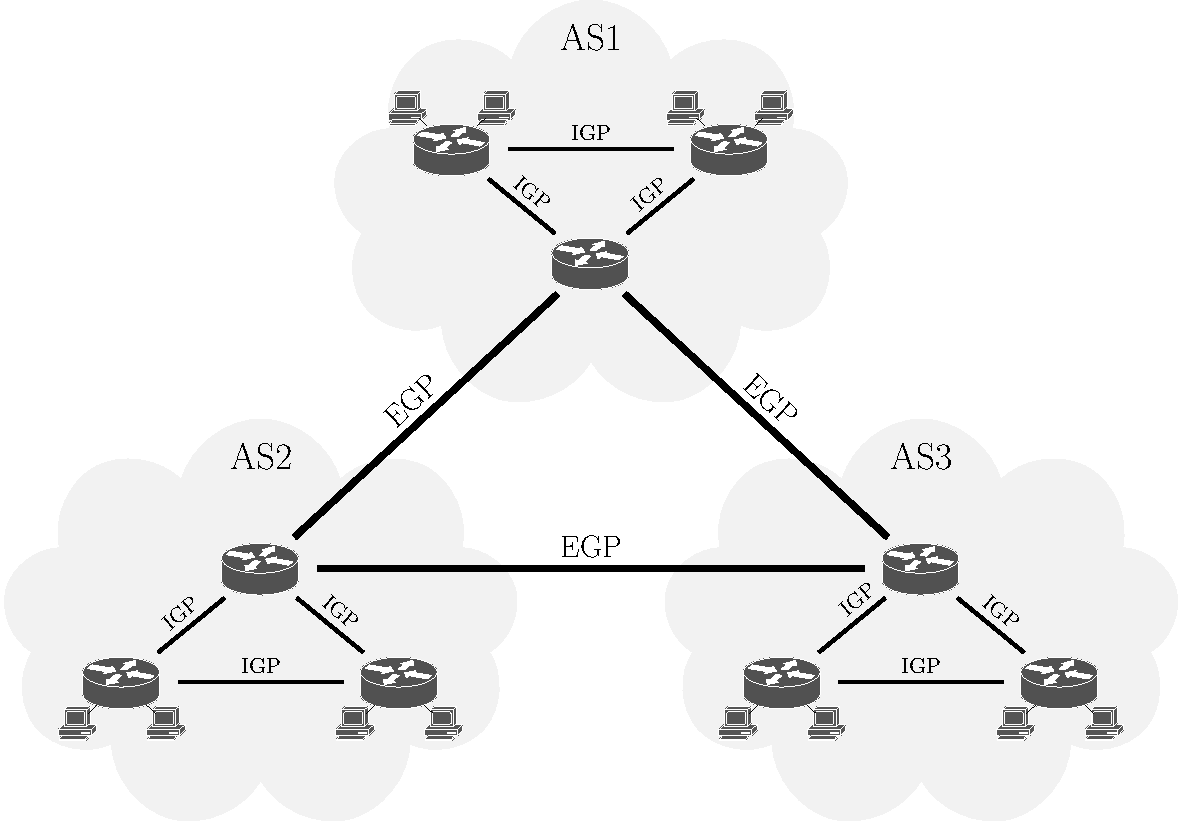
\includegraphics[width=.4\linewidth]{as}}\quad%
%   \subcaptionbox{\label{fig:layers}Network layers}{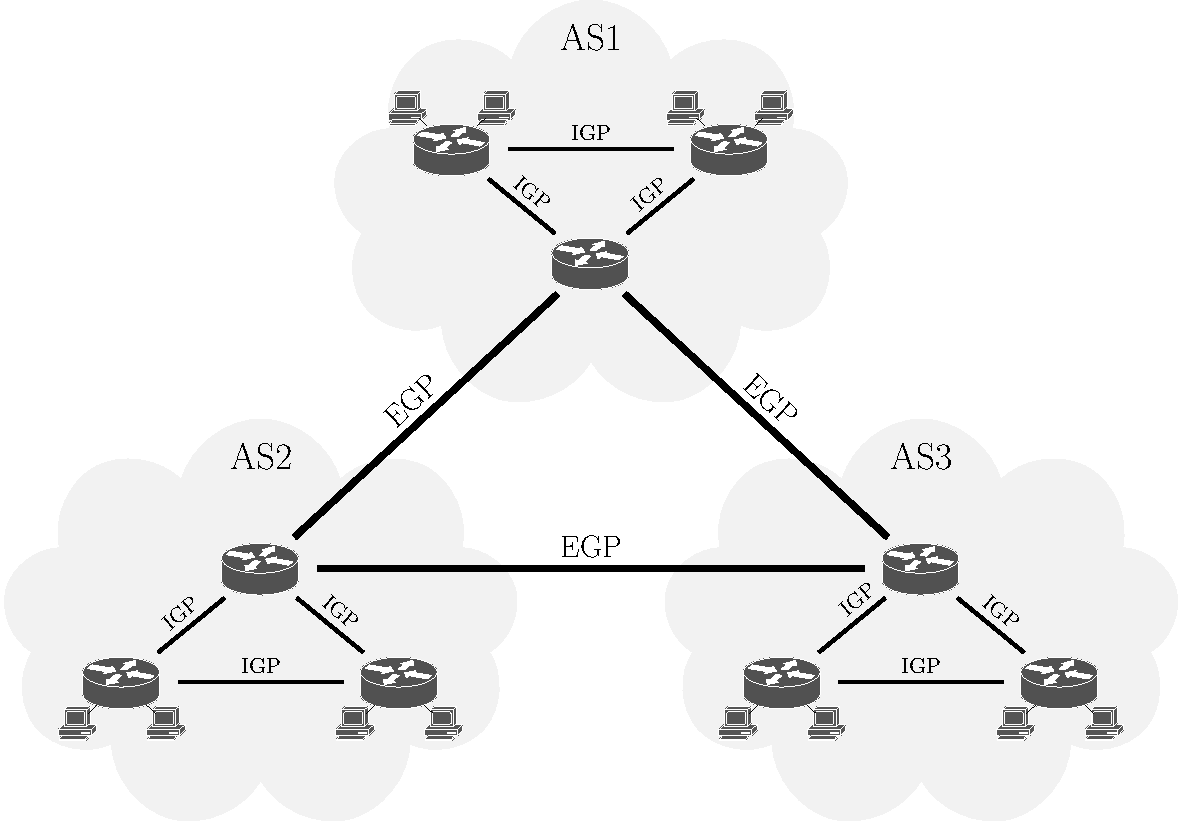
\includegraphics[width=.4\linewidth]{as}}%
%   \caption{WAN, MAN, CAN, LAN...\label{fig:as}}  
% \end{figure}

\begin{description}
\item[Is it covered by signal towers?] Signal tower is kind of hardware. It's not the only
  kind of hardware to build the Internet.  The Internet is mainly built from routers,
  switches.
\item[WAN is a large network, but router range small range.] Obviously the WAN is not
  built from cheap home routers you can google 'backbone network devices'.
\end{description}

\subsection{Ethernet}
\label{sec:ethernet}

% ***human analogy of ethernet?
% Right, it's part of the rfc1180. What exactly you don't understand about it?
% no good. when you say 'All of it', that means you haven't read it very carefully.
% you have to read it word by word, again and again, to find out where is the very hard point of understanding.

\subsubsection{Bus vs. Ring?}
\label{sec:bus-vs.-ring}

An Ethernet is a bus network. Topology?  Yes, it is. A ring network is also kind of
topology. What's the difference between ring and bus network?

Thanks to SUTRADHAR:
\begin{description}
\item[Ring] A ring topology is a network configuration in which device connections create
  a circular data path. Each networked device is connected to two others, like points on a
  circle. Together, devices in a ring topology are referred to as a ring network.
\item[Bus] A bus topology is a network setup where each computer and network device is
  connected to a single cable or backbone. Depending on the type of computer network card,
  a coaxial cable or an RJ-45 network cable is used to connect them together.
\end{description}

Yes, we know what a ring net looks like, and what a bus net looks like. But the key
difference between them is not how they look, it's how they work.

\begin{itemize}
\item Over a ring network how the nodes transfer data to each other? what the protocol
  should be?
\item Over a bus network, how the nodes communicate to each other? what the protocol should be?
\end{itemize}

The bus network is a broadcast network.  One node say something, all the other nodes can
hear. this is called broadcast.  The ring topology is not suitable for broadcast.  That
means the protocol used on bus network is not suitable for a ring network.  The protocol
used on bus network is CSMA/CD. it's well explained in rfc1180. you should have read
CSMA/CD already. If not, you read it, especially the human analogy part of CSMA/CD.

The protocol used on the ring network is \emph{token ring}. You should google that to see
how it works.

About Ethernet you need to know the following things:
\begin{itemize}
\item Address format, 6 bytes (48 bits) long
\item Broadcast address, \texttt{FFFFFFFF}
\item Ethernet frame format (Fig.~\ref{fig:eth-frame}). Looks like an envelop with
  something (IP packet, or ARP packet) inside.
\item CSMA/CD
\end{itemize}

\begin{figure}
  \centering
  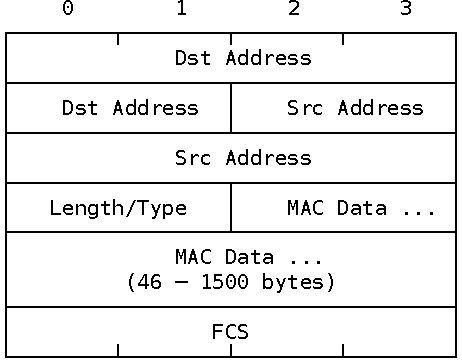
\includegraphics[width=.3\linewidth]{eth-frame}
  \caption{Ethernet frame format}
  \label{fig:eth-frame}
\end{figure}

% \subsubsection{Frame Check Sequence (FCS)}
% \label{sec:frame-check-sequence}

% \url{https://en.wikipedia.org/wiki/Frame_check_sequence}

% \subsubsection{CSMA/CD}
% \label{sec:csmacd}


\section{2020-05-11 Mon}

\subsection{Multiplexing and De-multiplexing}
\label{sec:mult-de-mult}

It's explained in RFC 1180. Data running in a cable is very much like water running in a
pipe.

\begin{itemize}
\item Multiplexing (n-to-1) means data come from many directions will go to only one
  direction.
\item De-multiplexing (1-to-n) means many different data come from one same path will go to
  different directions.
\item m-to-n is same as n-to-m, means there are many incoming data streams coming from
  many directions, each one of them will go to different directions.
\end{itemize}

For example, there are 10 people walking on the same road. This road is a
multiplexer because it serves 10 people. When these 10 people comes at a 10-way crossroad,
each one of them will go in a different direction. This is called de-multiplexing. One people
goes one way, no more multiplexing.

Read more carefully about the IP router part of rfc1180. IP module works in n-to-m mode.

\subsection{Encapsulation}
\label{sec:encapsulation}

You put your letter into an envelop, this is called encapsulation. The outgoing data
passing through the protocol stack will be encapsulated by each layer. That means it will
be encapsulated several times. It's very much like a set of nested
envelops \citetitle[Sec.~1.5.2]{kurose2013computer}.

\begin{itemize}
\item A TCP segment is an envelop with something (email message, chat message,
  etc.) inside. an UDP datagram is similar.
\item A IP packet is an envelop with something (TCP segment, or UDP datagram)
  inside.
\item A Eth frame is an envelop with something (IP packet, or ARP packet) inside.
\end{itemize}

\paragraph{What's interoperate and interoperability?}

You send a letter to me, then I send you some feedback. This is called interoperate.
You say something to me, I never feedback. This is not interoperate.
Interoperability? That's the ability to interoperate.

\subsection{IP layer}
\label{sec:ip-layer}

\paragraph{Do IP routers have any TCP or UDP module?}

Yes. There are TCP/UDP and application layers in IP routers though it's not strictly
necessary. Without the application layer, there is no way to configure the routing table
which is the core inside the IP module.

The IP module is very much like a post office. Usually, the letters coming into a post
office are not destinated to the post office. Rather, the letters are supposed to be
forwarded by the post office to somewhare else. In most cases, the post office doesn't need
to open the letter to see the contents inside. The post office just needs to check the
destination address written on the envelop.

In the real world, a letter's journey from the sender to the receiver takes several steps.
\begin{enumerate}
\item The sender
  \begin{enumerate}
  \item puts the letter into an envelop, and write the recipient's address on the
    envelop.
  \item drop it into a postbox.
  \end{enumerate}
\item The post system
  \begin{enumerate}
  \item The postman takes your letter to the post office.
  \item Some staff in the post office checks the destination address on the envelop to see
    where it should be forwarded.
  \item Put it (together with other letters with the same direction) on a car/train/air
    plane traveling to the next hop (post office)
  \item At the next hop, the destination address is checked again to see where it should
    be forwarded.
  \item The above steps repeat at each hop until the letter arrives at the last hop.
  \item A postman will take this letter to the destination address, and put it in the mailbox.
  \end{enumerate}
\item The receiver
  \begin{enumerate}
  \item Checks to see if this letter addresses to me? If it is,
  \item Opens it.
  \end{enumerate}
\end{enumerate}

The Internet works very much like the post system we described above.
\begin{itemize}
\item The senders and the receivers are the application programs at the end computers.
\item Routers work in a similar way to post offices.
\end{itemize}

\paragraph{What's end-to-end transmission?}

For example, when you send an email to a friend, the program you've been using to send the
email is one end of the transmission. When the email arrives the destination, your friend
opens it with another email program which is the other end of the transmission. So,
end-to-end transmission is program-to-program transmission. The \emph{post offices} in
between are not \emph{ends}, they are \emph{hops}. The email travels from one end to
another end in a hop-by-hop manner.

\subsection{IP Address}
\label{sec:ip-address}

\paragraph{Why my IP address changes every time upon a restart?}
\label{sec:dhcp}

If you stay at one place, e.g. you home, all the time, then usually your IP address won't
change every time you restart your computer, because the DHCP server in your home router
can remember this computer. It will try allocate the same IP to it every time.  You IP
address is dynamically allocated by the DHCP server.

\paragraph{How to find out which class an IP address belongs to?}
\label{sec:ip-addr-class}

You can figure it out by doing some calculation.  It's not so easy to calculate. So you
can use some tools to help you. For example, on Linux, we have a command \emph{ipcalc}, by
which you can type, for example ``\texttt{ipcalc 192.168.8.8}'', to see its details.

There are many web resources talking about IP address classes. For example, 
\url{http://techiebird.com/networkclass.html}

\section{2020-05-13 Wed}
\label{sec:2020-05-13}

No questions? Here's my question. You've finished reading RFC 1180, haven't you? And you
don't have any questions. Then, you should be able to describe the whole process in which
an email is transferred from one computer to another. In figure~\ref{fig:routing}, tell me
\begin{description}
\item[Question 1:] How an email is transferred from host Alpha to host Beta?
\item[Question 2:] How an email is transferred from host Alpha to host Epsilon?
\end{description}

This question will appear on your exam paper. And it's worth at least 20 points.

\begin{figure}
  \centering
  \includegraphics[width=.8\textwidth]{indirect-routing-2}
  \caption{A campus network\label{fig:routing}}  
\end{figure}


\end{document}
%%% Local Variables:
%%% mode: latex
%%% TeX-master: t
%%% End:
